%!TEX root = ../../thesis_master.tex

%%%%%%%%%%
\chapter{Implementation}
\label{chap:implementation}
%%%%%%%%%%

In this chapter the 

\section{Gazebo Simulation}
\label{sec:gazebo-simulation}

It has been already explained how ROS works as an operating system for the robot, allowing the complete implementation of a robotic system. This is valid not only for real hardware, but also for simulated robots. In order to do that, an additional tool is needed to work in together with ROS. This is the roe of the \emph{Gazebo} robotics simulator.

\emph{Gazebo} is a 3D dynamic simulator used to simulate robotic environments. It allows the simulation of the kinematic and dynamic simulation of robots and other bodies, indoor and outdoor environments with different illumination conditions and textures and the emulation of sensors such as cameras or light rangers. Additionally, using the \emph{Gazebo} plugins it is possible to model more complex phenomenas including aerodynamics or controllers.

\emph{Gazebo} works as an additional ROS node. It subscribes to the topics containing the robot's current state and publishes in other topics the new state of the robot. 

\begin{figure}[!htb]
	\caption{Example of simple communication between Gazebo and ROS}
	\centering
	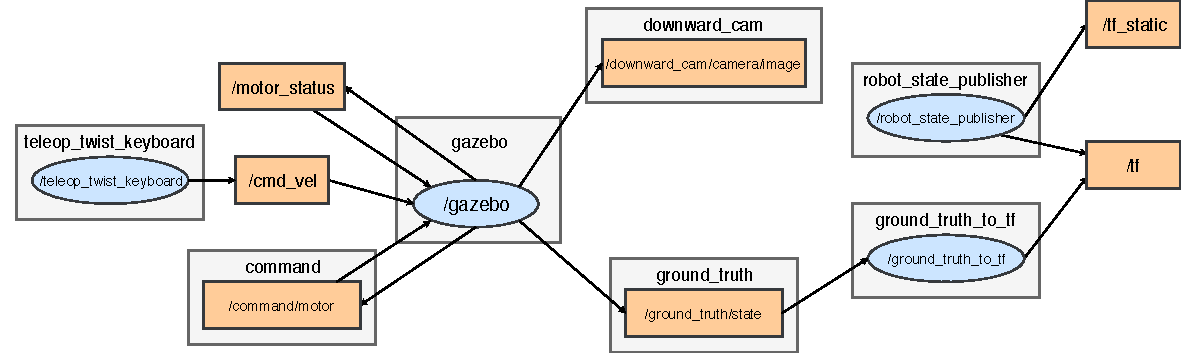
\includegraphics[width=\textwidth]{content/chapter_05/images/gazebo_example.pdf}
	\label{fig:gazebo_example}
\end{figure}

\section{Visp Visual Servoing Framework}
\label{sec:visp}

\section{AprilTag Markers}
\label{sec:apriltag_markers}

\section{ROS Actions}
\label{sec:ros_actions}
